\documentclass[12pt]{article}
\usepackage[T2A,T1]{fontenc}
\usepackage[utf8]{inputenc}
\usepackage[greek,russian,english]{babel}
\usepackage{mathpazo}
\renewcommand{\familydefault}{\rmdefault}
\usepackage[landscape,a4paper]{geometry}
\geometry{verbose,tmargin=0cm,bmargin=0cm,lmargin=3cm,rmargin=3cm}
\usepackage{fancybox}
\usepackage{calc}
\usepackage{multicol}
\usepackage{graphicx}
\usepackage{url}
\usepackage{eso-pic}
\usepackage{textcomp}
\usepackage{paratype}
\usepackage{tgpagella}


\DeclareFontFamilySubstitution{T2A}{\rmdefault}{PTSerif-TLF}

\newcommand\BackgroundPic{%
\put(0,0){%
\parbox[b][\paperheight]{\paperwidth}{%
\vfill
\centering
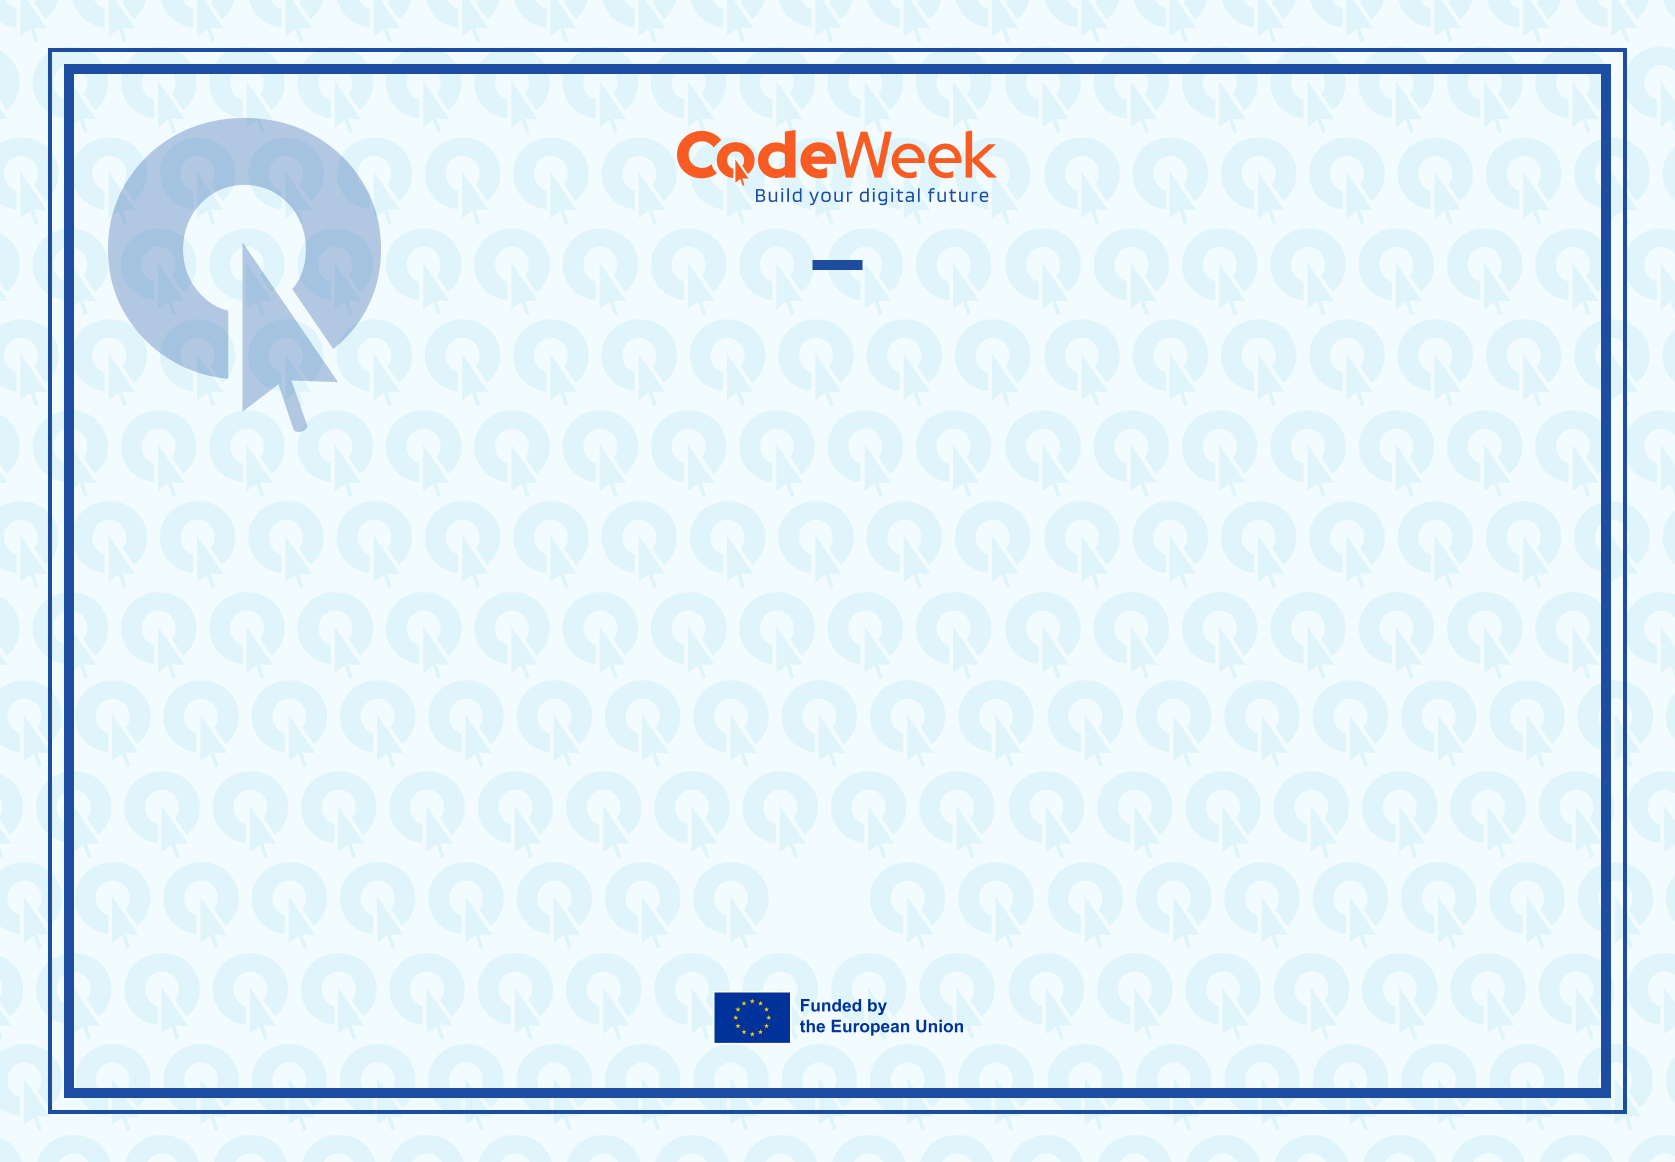
\includegraphics[width=\paperwidth,height=\paperheight,%
keepaspectratio]{images/participation-certificate-2025.png}%
\vfill
}}}


\begin{document}
\AddToShipoutPicture{\BackgroundPic}
~
\vspace{3.5cm}
~
\begin{center}

\begin{table}[h]
\footnotesize
\begin{center}
\begin{tabular}{lr}
%~\hspace{0.7cm}
\end{tabular}
\end{center}
\end{table}
\vspace{-0.2cm}
\LARGE{CodeWeek EU organisers are honoured\\
\vspace{1cm}
\fontsize{40}{50}{\textbf{TO CERTIFY}}
}

\vspace{0.4cm}

\Huge{that
\begin{otherlanguage*}{russian}
\textbf{<CERTIFICATE_HOLDER_NAME>}
\end{otherlanguage*}
}


\vspace{0.4cm}

\Huge{actively contributed to the success of}

\vspace{0.3cm}

\Huge{\textbf{EU Code Week <CERTIFICATE_YEAR>}}

\vspace{0.3cm}

\Large{by running a coding event.}

\vspace{.2cm}

\vspace{1cm}

\begin{table}[h]
\footnotesize
\begin{center}

\end{center}
\end{table}

\vspace{-3cm}
\end{center}
\begin{table}[h]
\footnotesize
\begin{center}
\begin{tabular}{lr}
%~\hspace{0.7cm}
\includegraphics[height=2.5cm]{images/signature_and_stamp.png}
\end{tabular}
\end{center}
\end{table}
\vspace{-1.2cm}
\begin{center}
\footnotesize{On behalf of EU Code Week Ambassadors}\\
%\end{tabular}

%Diploma elaborado con el software libre \texttt{Pyploma}, (c)
%\url{fjruizruano@gmail.com} bajo licencia
%GPLv3. Visite: \url{http://code.google.com/p/pyploma}

\end{center}
\end{document}
